\section{Evaluation of a traceability solution}\label{sec:evaluation}
\sideboxbegin{o}
This section presents a protocol to evaluate traceability solutions and answers whether Capra is a valuable generic solution for traceability. 
\sideboxend

The quality traceability solutions lies on five main pillars : 
(1) The customization of the tool to adapt to different systems\footnote{We call \textit{system} or \textit{software system} interchangeably here, considering a software system an abstract representation of a (software) system.}, 
(2) the level of automation of the identification of traces, 
(3) the means of visualisation and retrieval of trace links, 
(4) the means of persistence and additional operations available, 
(5) and the quality of its constituents.
In this section, we present a protocol for the evaluation of traceability solutions following these dimensions and explore them independently. We detail the application of the protocol to Capra (see below) and how this latter responded.

\begin{descriptioncompact}
    \item[Quick presentation of Capra] Capra is a tool and a research project aiming at generic software traceability \cite{heisig2019-generic-traceability-metamodel-end-to-end-capra,maro2016_maintenance_factors_and_guidelines}. Its initiators rose the ability to trace as a noticeably important feature to integrate into the realm of model-driven engineering.  Scientific publications show that strong traceability has been long due in the field and distinguish themselves from other approaches with an important focus on customizability and visualization of tracing artefacts \cite{clelandhuang2007bestPracticeForAutomatedTraceability,mader2010-visual-tracability-modeling-language}. The overall goal of Capra is to allow the linking of elements from different domain specific modeling languages.

    The implementation is based on the Eclipse Modeling Framework \cite{EMF} hosted open on Git \cite{Capra_Repo}. It consists in an Eclipse plugin that carries out the requirements an industrial partner mandates. There is a core plugin, which grows around new adapters to more and more domain specific languages. To quote but one example, Capra is ready to use with Papyrus models and elements. 
\end{descriptioncompact}

\subsection{Evaluation protocol}
Table \ref{tab:evaluationtable}, summarizes the five steps of the evaluation protocol.

\begin{table}[h]  
	\centering
	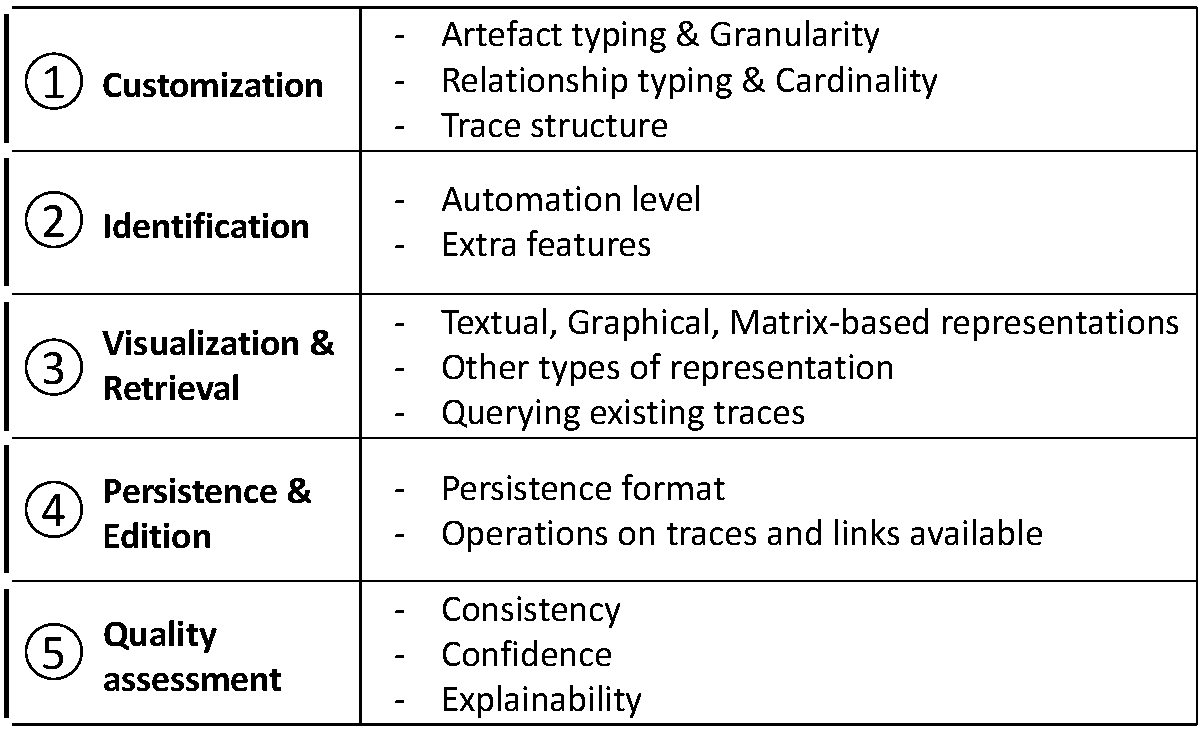
\includegraphics[width=.65\linewidth]{images/evaluation-table.pdf}
	\caption{Five pillars for traceability evaluation.}
	\label{tab:evaluationtable}
\end{table}

 
\begin{enumerate}
    \item First, to evaluate the potential a tool has to address a specific purpose, \textbf{customizability} must be evaluated with regard to the kind of artefacts and the kind of links it offers to manipulate\footnote{We call trace links, connections, relationships, simply \textit{links} in this document, as opposed to \textit{trace} which are entities composed with (successive) links.}. Generic tooling must allow an \textit{ad hoc} definition of types to adapt to different uses in different application domains \cite{maro2016_maintenance_factors_and_guidelines}. 
    
    \item Then, how is the identification process? The identification of traces can be automated to different levels. Links can be identified manually as well, which usually depends on the integration of the tool into the system's environment. 
    There exists explicit links in the syntax trees of many languages. These can be automatically derived, included or used only for visualization as an extra feature (or known neighborhood). 

    \item Once traces are identified, they can be represented in textual or graphical form, revealing their structure in a (more or less) legible way, and editable to a certain degree. Matrix-based representations show a broader aspect of the traces in a more "conventional" way that some favor \cite{li2013-trace-matrix-analyzer}. 
    
    \ughu{ What are the mechanisms to retrieve existing traces? Is there a system to query them?} 

    \item \ughu{Persistence format of tracing elements. Textual expressiveness? SQL efficiency? XML interoperability? 
    
    Traces are complex entities and a robust tooling should also offer robust operations to handle them with precision and efficacy.}
    
    \item Finally, how is the quality of the trace and its constituent assessed? Traces suffer gradual decay, depending on the degree of versatility of the system, they might not be kept up-to-date, and their consistency with the system's artefacts may decline. This indicates that traces might suffer some uncertainty. Is the confidence into the degree of existence of a trace is evaluated? If a trace has been identified automatically, traces should refer to evidences about the rationale behind their identification. Is the tool offering any means to express these considerations?
\end{enumerate}


%What is the nature of the entities one wants to trace? There will be different types of artefacts to target and the relationships between these artefacts may vary significantly. To adapt to the different goals traceability can be used for, Capra allows a custom definition of the artefacts' and relationship' types.  

\Fig{fig:evaluationpoints} schematizes the traceability infrastructure. It shows the three main components: the traces and their constituents, the environment in which it \ughu{functions}, and the artefacts it targets on (a) system (of systems). 
 
\begin{figure}[h]  
	\centering
	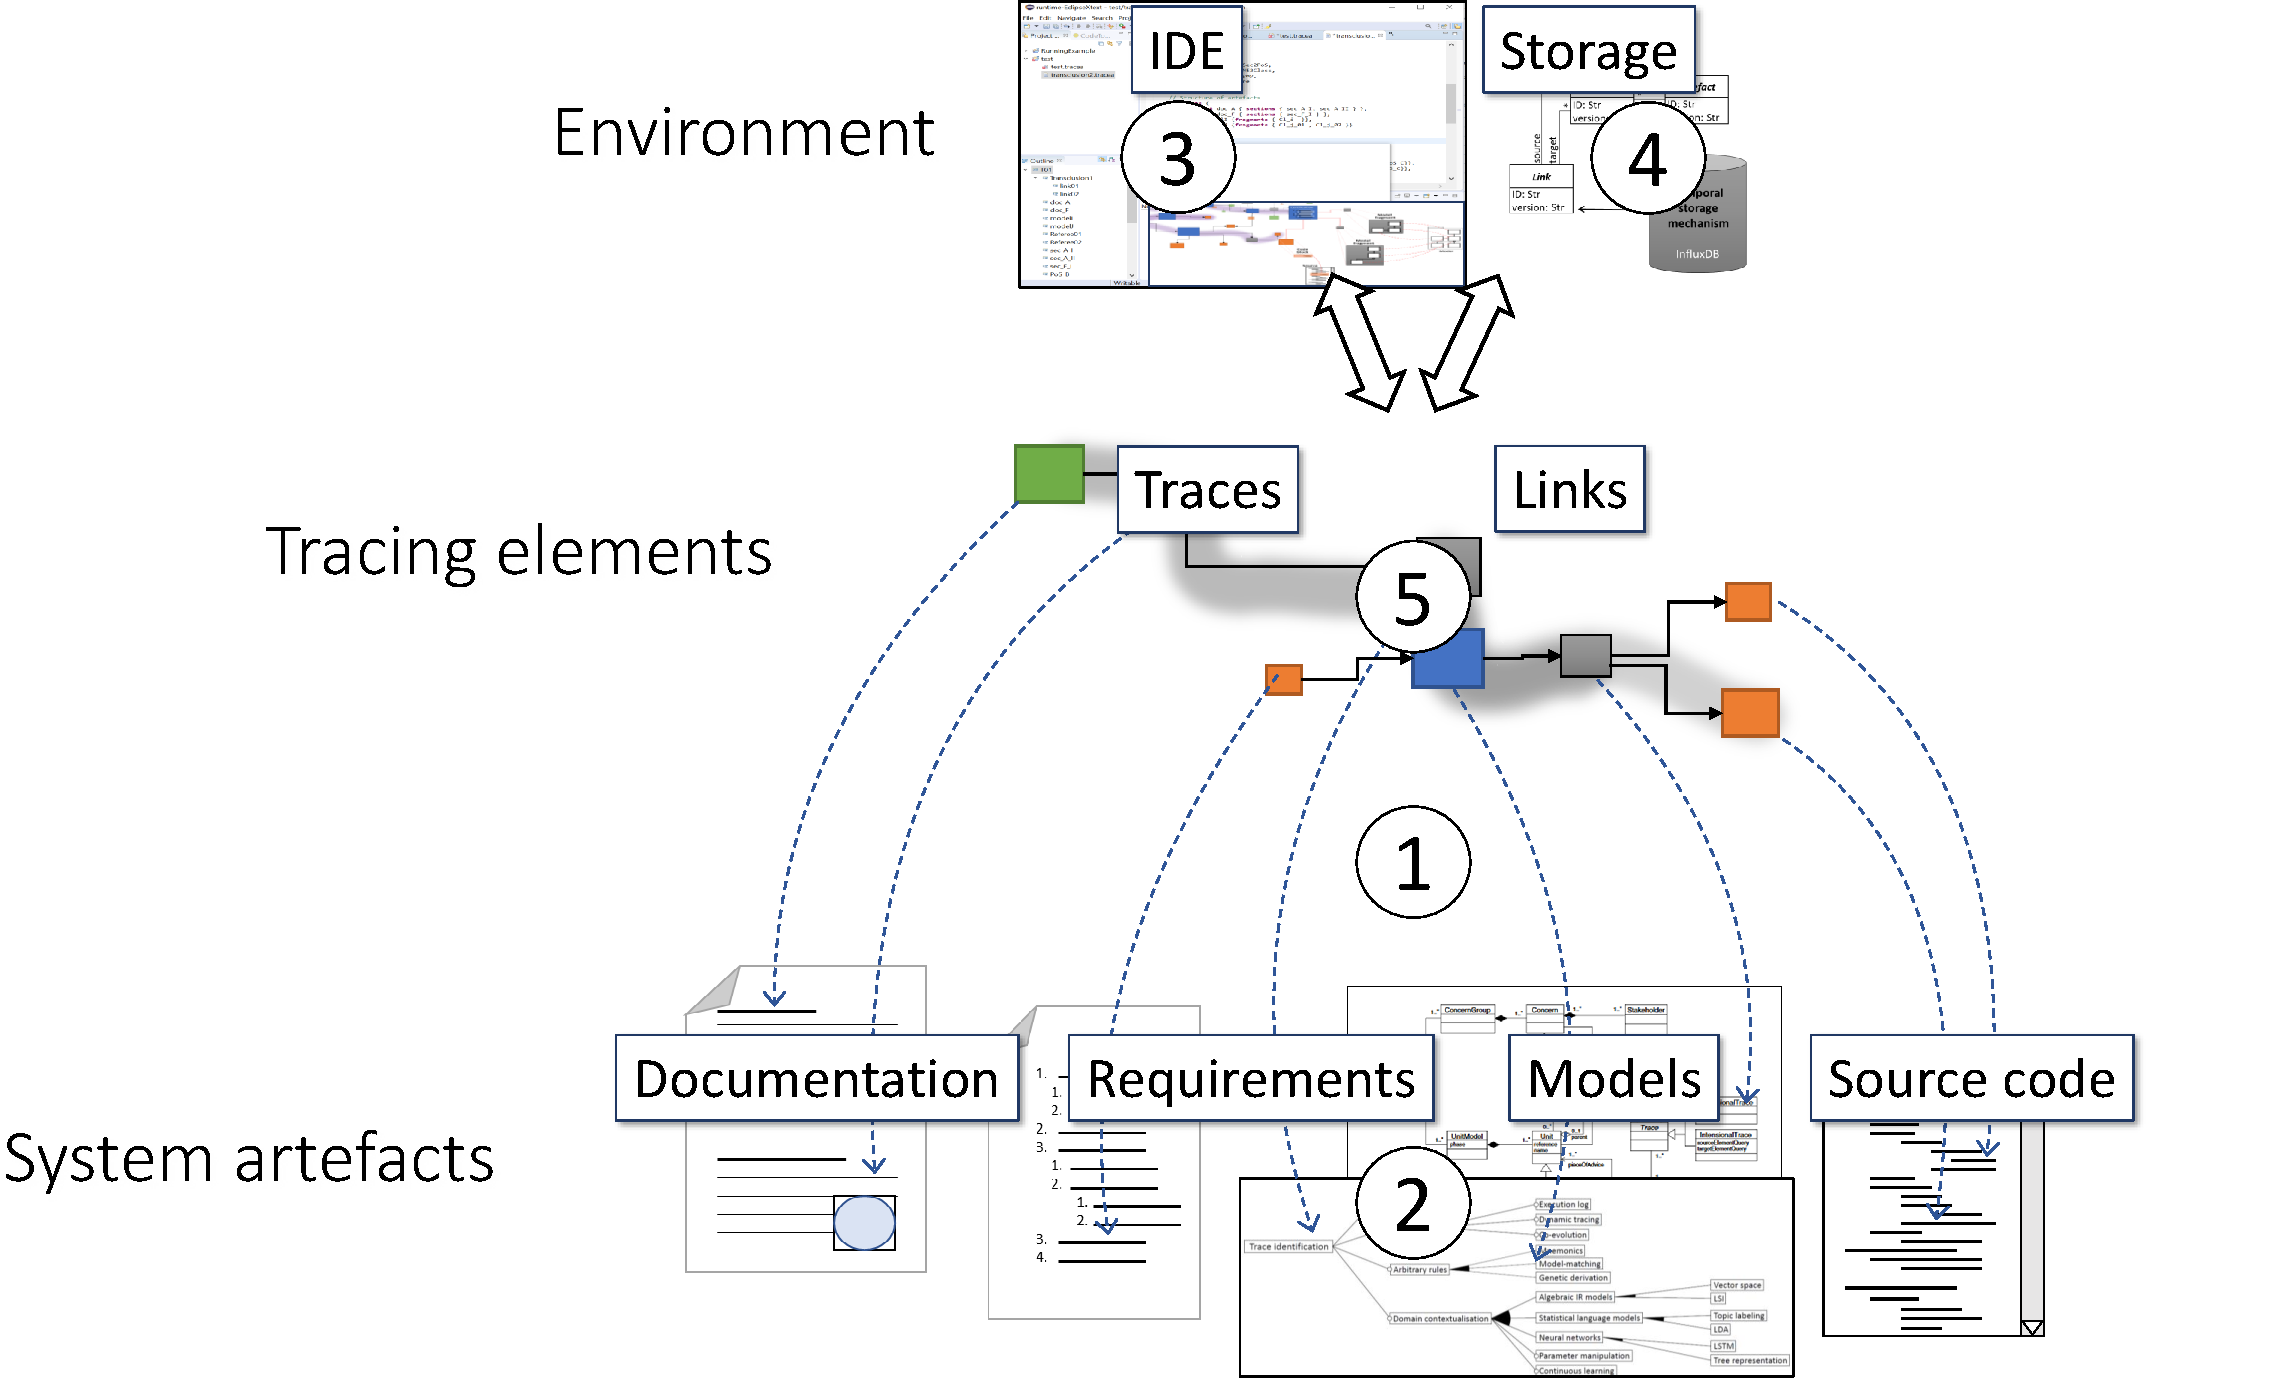
\includegraphics[width=.85\linewidth]{images/evaluation-points.pdf}
	\caption{Points of interest for the evaluation of traceability}
	\label{fig:evaluationpoints}
\end{figure}



\subsection{Traceability customization}\label{sec:custom}

Capra allows a custom definition of the artefacts' and relationship' types.  The customization of artefacts and links is editable through an XCore plugin.  Links can be defined following a hierarchical inheritance and allowing structural features (reference and attributes)\footnote{There is no guaranty on the level of implementation of the more complex features XCore allows.}. 
Capra is an EMF plugin and benefits from the artefacts the instance of the platform is running on. An artefact is defined through the resource change management plugin mechanism of EMF infrastructure. The wrapping of the artefacts uses another XCore plugin to allow the definition of other attributes for artefacts: \verb|org.eclipse.capra.generic.artefactmodel|.
The adapters, handlers, and helpers for the EMF artefacts must be redefined as Java polymorphic overriding projects (derived from \verb|org.eclipse.capra.generic.core|).  
Capra redefines wrappers for 15 languages or standards such as UML, BPMN, Papyrus, Mylyn, Java, C++ Office, to name a few\footnote{There is no documentation relating the means to apply such redefinition - neither can be found any tips on the potential impact such changes may initiate.}. 
In the default implementation, links are part of a \texttt{TraceModel} that \textit{connects} between them. There is no explicit trace structure. 
If an artefact is part of the target of a link and the origin of another, the trace connects (see the Section \ref{sec:visualization} on visualization). By default there is one generic \textit{RelatedTo} possible kind of link. For each link, there must be one and only one source and one or more target artefacts.
The default \texttt{GenericTraceModel} implementation must be transferred or adapted (Java file, no documentation) to be adapted to a new structure. There is no test coverage for potential alterations to the original implementation.


\subsection{Links identification}\label{sec:identification}
Identifying links in Capra is done manually. Any element actionable in an Eclipse environment can be selected to take part of a trace. A context menu reacts to elements and offers to add to the "Traceability selection", or drag-n-drop the element into the \texttt{Trace Creation}\footnote{Names are subject to change.} view. (Respective adapters are required, see Section \ref{sec:custom}.)
There is no automation for the identification of custom relationships, but the UML dependencies can be viewed in the \texttt{Capra PlantUML Viewer}. UML relations are not part of the synthesis of the trace links. They are derived for (visual) convenience and they need to be manually recorded to be synthesized.


\subsection{Trace visualization \& retrieval}\label{sec:visualization}
Capra offers different visualization options:
	
\begin{descriptioncompact}
    \item[Augmented text representation of links] 
Traces in Capra are synthesized into XMI Ecore models. This is convenient for Eclipse offers a \texttt{Reflexive Ecore Model Editor} to browse and edit such resources. Traces themselves cannot be apprehended though, if not to a great cost, because this view do not show the succession of trace links. \Fig{fig:xmieditor} shows a screenshot of this view. As can be seen, a name composed with the name of the artefacts targeted is the only information available - together with the elements in the \texttt{Properties} view associated. 
Instances of the wrappers for the artefacts used by the trace links are stored in the same manner in another file.
\begin{figure}[h] 
	\centering
	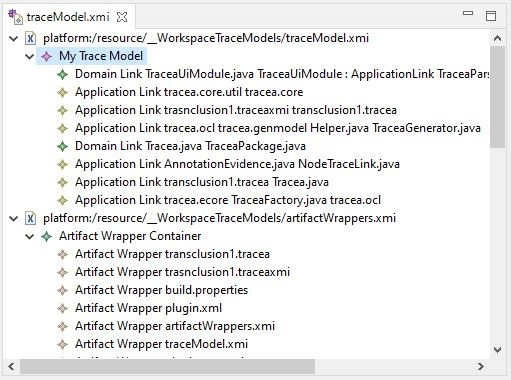
\includegraphics[width=.65\linewidth]{images/XMIEditor.jpg}
	\caption{Links are browsed with Eclipse Ecore editor}
	\label{fig:xmieditor}
\end{figure}

    \item[Graphical representation of traces] %using PlantUML/GraphViz plugin
To ease the visualization, Capra generates a graphical description of traces in the \missref{GraphViz} languages and uses \missref{PlantUML} to plot them in an Eclipse view. Figure \ref{fig:plantuml} shows a capture of the view.
This view shows the links associated to the element selected in the Eclipse IDE. These links are the one \ughu{identified} with Capra (the trace links) or are derived from the neighborhood of the element selected. In the case of a Java class, a type hierarchy is provided.
The view is configurable. The type of links, as well as \ughu{the depth of their transitivity} can be changed through the Eclipse interface.  
\begin{figure}[h] 
	\centering
	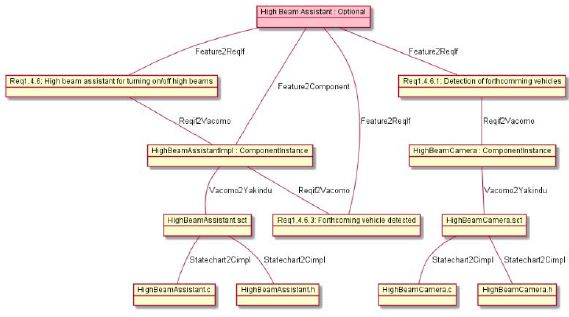
\includegraphics[width=.60\linewidth]{images/plantuml-viewer.jpg}
	\caption{Trace links sequences are plotted graphically in Capra PlantUML Viewer}
	\label{fig:plantuml}
\end{figure}

    \item[Matrix-based representation of tracing] 
Numerous authors in traceability shows the importance of a \ughu{broader} point of view on the tracing process that shows the linkage between the traced artefacts through an association matrix. The Capra solution offers an association matrix view, as can be seen in \Fig{fig:matrixviewer}. It can be exported in the Excel (xls) format.
\begin{figure}[h] 
	\centering
	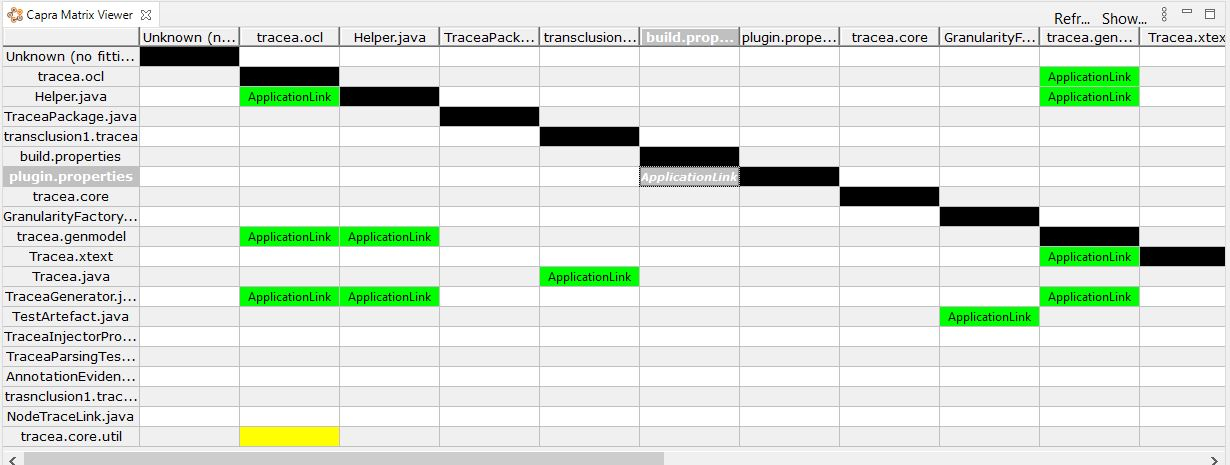
\includegraphics[width=.65\linewidth]{images/matrixViewer.jpg}
	\caption{Interrelations can be viewed in the matrix-based representation}
	\label{fig:matrixviewer}
\end{figure}

    \item[Link retrieval] There is no mechanism to retrieve automatically trace links. Yet, the use of \missref{IncQuery} is a strong bet to address this limitation for it is tailored to query XMI Ecore resources.
\end{descriptioncompact}


\subsection{Trace persistence \& edition}
Traces are synthesized into an Ecore model, stored in an XMI file. Artefacts wrappers are also stored in XMI.
The \texttt{Reflexive Ecore Model Editor} (together with the \texttt{Properties} view, see  \Fig{fig:properties}) can be used to edit the information but the consistency of other views is not guarantied. Eclipse must be closed and reopened.
The name of the files appear in the project list, but their name cannot be edited.
\begin{figure}[h] 
	\centering
	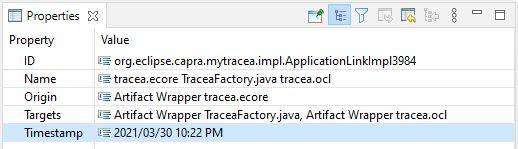
\includegraphics[width=.65\linewidth]{images/properties.jpg}
	\caption{Links are viewed and edited with Eclipse Properties view}
	\label{fig:properties}
\end{figure}

\subsection{Trace quality evaluation}
Capra checks the consistency of traces when artefacts are modified or deleted through the Eclipse platform. Changes in the software elements triggers a validity check on the links these elements take part (as source or target). If there is a consequence, the links are tagged with a warning. There is no fix proposed.

Confidence is not quantified and there is no record of the facts or evidences about the existence of a link.

\subsection{Conclusion}

Table \ref{tab:evaluationcapra} summarizes the evaluation of Capra. As can be seen, the tool benefits a strong customization potential: it is easy to design wrappers for new artefacts with Eclipse \texttt{IResource} redefinition, and the definition of link types is very expressive thanks to XCore. If the tool lacks some automated mechanisms to identify traces, the visualization of both specific links and derived UML relations is \ughu{intriguing}.
Unfortunately, the tool also suffers important limitations. We depict them in the next section. 


\begin{descriptioncompact}
    \item[Customization ++]  (left the ui limitation for complex structures (ex: Evidences))
    \item[Visualization ++] (left the absence of interaction, it's all here to implement though)
    \item[Eclipse integration] benefits from the integration in EMF are significant : XCore expressiveness, ready made UI, \ughu{other plugins for Ecore}
\end{descriptioncompact}

\begin{table}[h]  
	\centering
	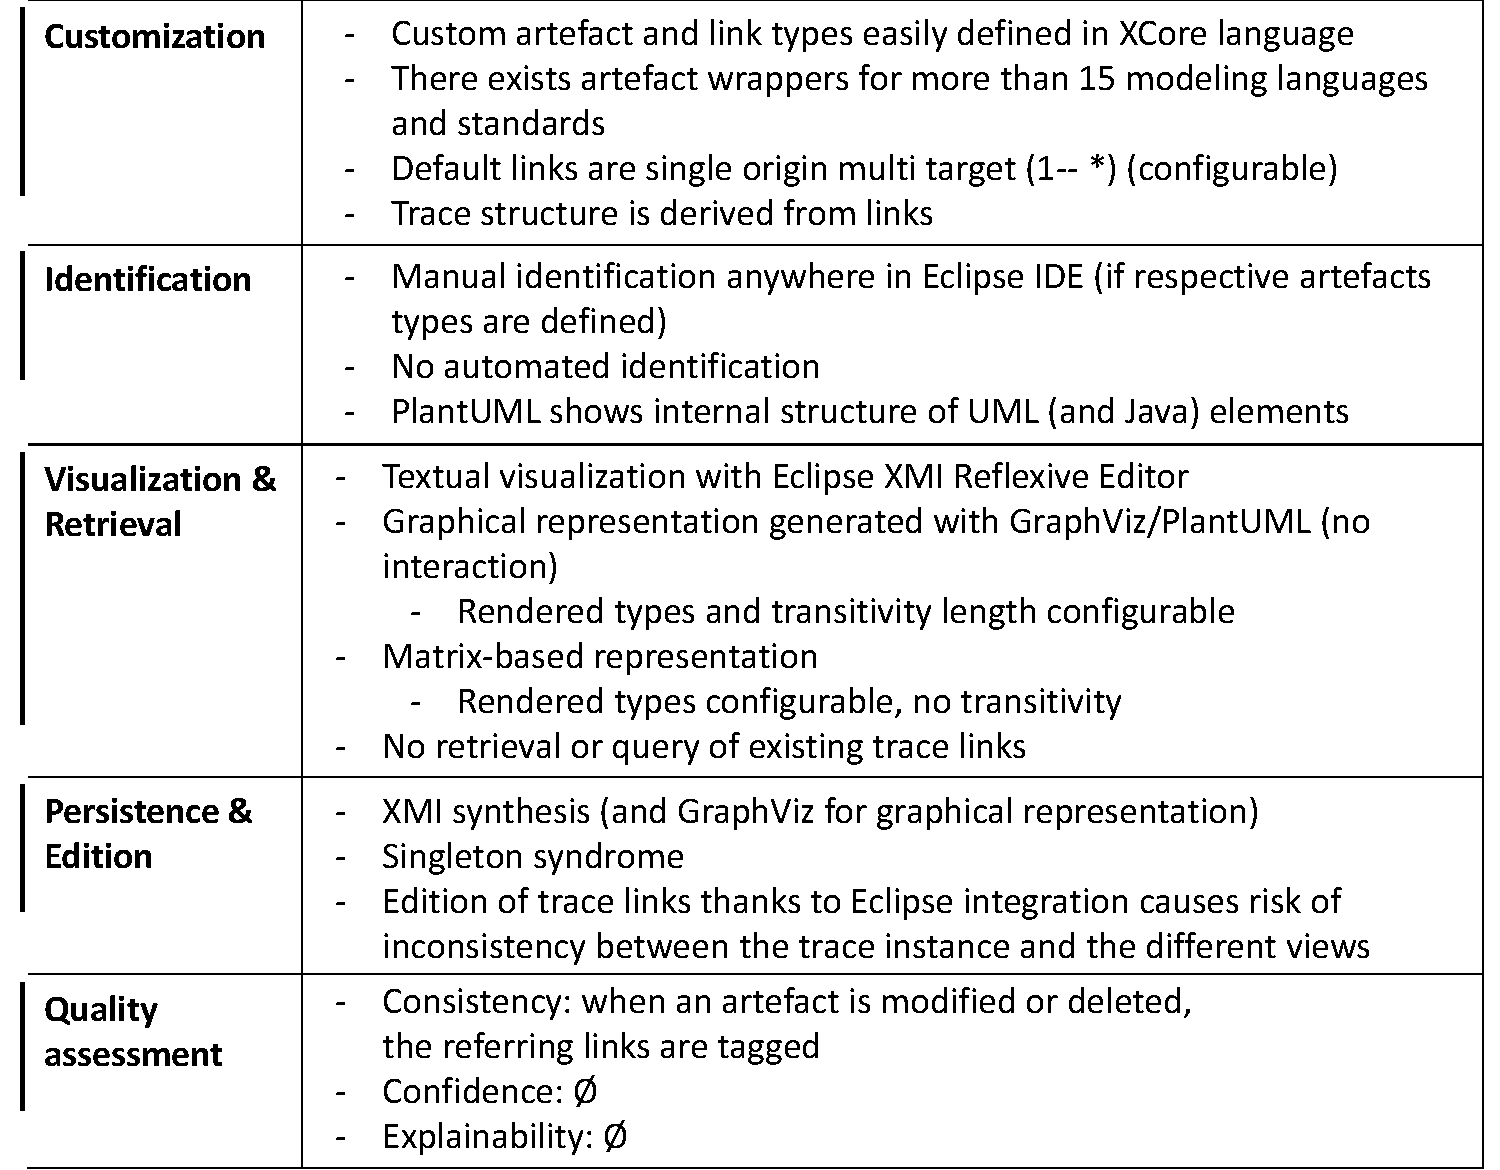
\includegraphics[width=.99\linewidth]{images/evaluation-table-capra.pdf}
	\caption{Summary of the evaluation of Capra}
	\label{tab:evaluationcapra}
\end{table}


